\section{RESULTADOS}
% APENAS PARA ILUSTRAR O TIPO DE PLOTS QUE PRETENDO COLOCAR
% CONSIGO REFAZER QUALQUER PLOT FACILMENTE
% TENHO INFORMAÇÃO/DADOS PARA GERAR DIVERSOS PLOTS E TESTES OFFLINE

% OBJETIVO:
% 1) MOSTRAR O RESULTADO DA CALIBRAÇÃO (CURVA ESTIMADA X DADOS BRUTOS)
% 2) MOSTRAR O RESULTADO DA FILTRAGEM; COMPARAR COM FILTOS SIMPLES (POSSO APLICAR OS FILTROS OFFLINE NOS DADOS COLETADOS)
% 3) MOSTRAR O RESULTADO DO CONTROLE, PRINCIPALMENTE COM O INTUITO DE DIMINUIR AS ASSIMETRIAS DOS MOTORES

% MOSTRAR:
% RESPOSTAS PARA DIFERENTES CONFIGURAÇÕES DE MOTOR-SENTIDO E COM DIFERENTES REFERENCIAS/SINAIS DE CONTROLE PARA:
% CURVA ESTIMADA X SEM FILTRO X COM FILTRO
% 


\subsection{Resultados da calibração}

\begin{figure}[H]
    \centering
    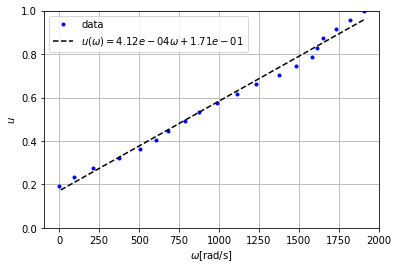
\includegraphics[width=13cm]{graficos/plot_test_calibration_result_feedforward.png}
    \caption{TESTE: RESULTADO DA IDENTIFICAÇÃO/CALIBRAÇÃO}
\end{figure}

\begin{figure}[H]
    \centering
    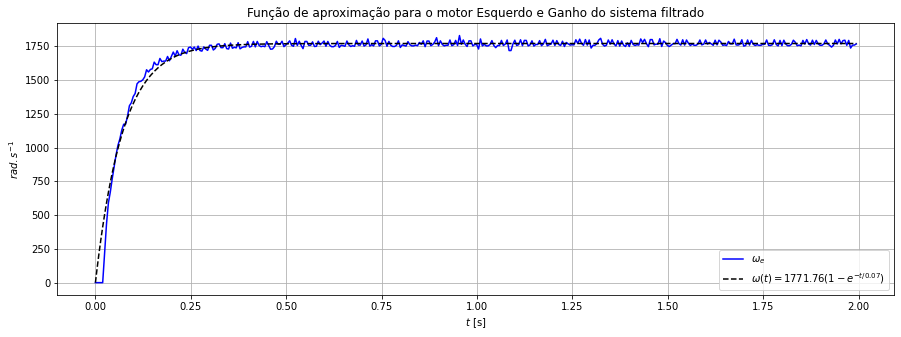
\includegraphics[width=13cm]{graficos/plot_test_identificacao.png}
    \caption{TESTE: RESULTADO DA IDENTIFICAÇÃO/CALIBRAÇÃO}
\end{figure}

\subsection{Filtragem da velocidade}
% MOSTRAR A FILTRAGEM COM DIFERENTES PARÂMETROS:
% sintonizando a incerteza da medição e do modelo (Q e R)

\begin{figure}[H]
    \centering
    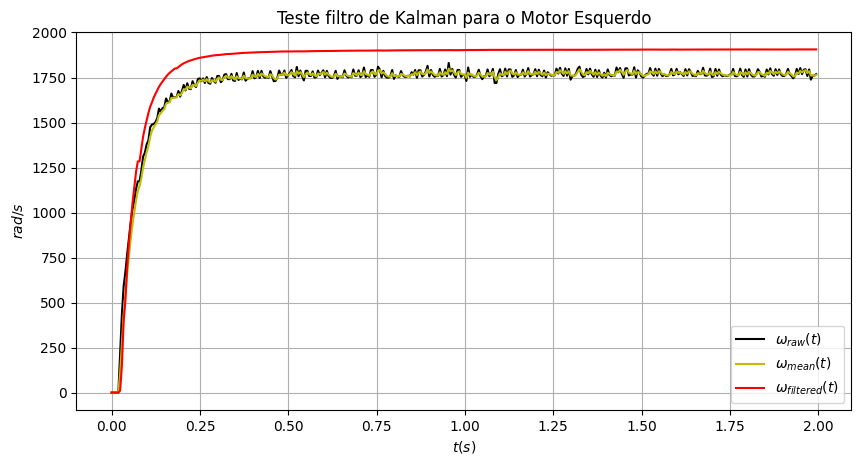
\includegraphics[width=13cm]{graficos/plot_test_media_x_kalman.png}
    \caption{TESTE: MEDIA VS KALMAN}
\end{figure}

\subsection{Respostas do sistema com os controladores}


\begin{figure}[H]
    \centering
    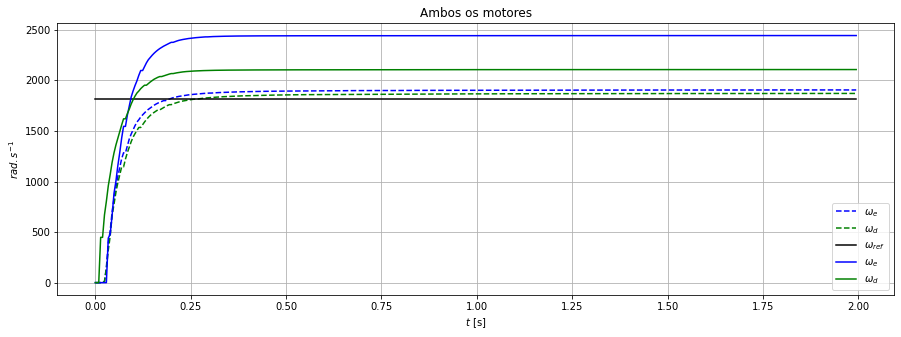
\includegraphics[width=13cm]{graficos/plot_test.png}
    \caption{TESTE: COM CONTROLE VS SEM CONTROLE}
\end{figure}

\begin{figure}[H]
    \centering
    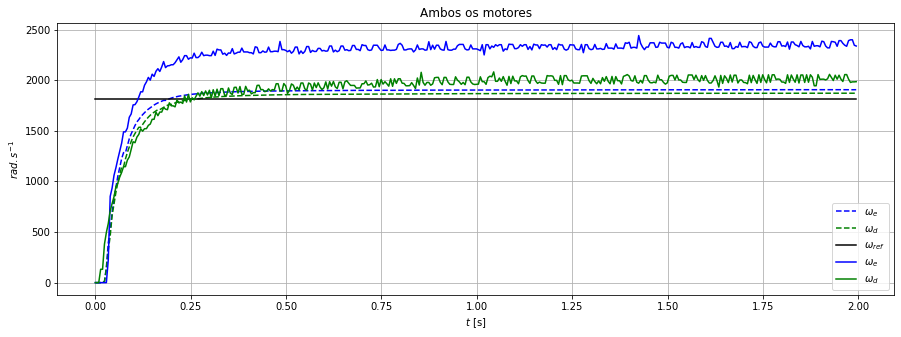
\includegraphics[width=13cm]{graficos/plot_test_antes_x_depois.png}
    \caption{TESTE: ANTES X DEPOIS}
\end{figure}